\chapter{\prizm~Instrumentation}
\section{\prizm~Experiment Overview}

\prizm~\citep[]{2019JAI.....850004P} shown in Figure~\ref{Fig:prizm} is an experiment that is specifically designed to study cosmic dawn in the universe using total power measurements of the global 21 cm signal from neutral hydrogen, redshifted to \SIrange{30}{200}{\mega \hertz}. The experiment consists of two compact, modified four-square antennas \citep{8072391} that operate at central observing frequencies of 70 and 100~MHz. The combined frequency range of both antennas spans \SIrange{30}{200}{\mega \hertz}, which brackets the predicted absorption feature from cosmic dawn. Figure~\ref{Fig:PRZIM_block} shows the subsystems of \prizm\, which will be discussed briefly, followed by a discussion on revised subsystems. The first installation of \prizm\ in Marion Island was in 2017, and over the years, there have been incremental upgrades and maintenance to the front and back end electronics. My main contribution was making additional upgrades that were planned to field during the 2020 Marion takeover voyage, which unfortunately did not happen because of the COVID-19 restrictions.

\begin{figure}
	\centering
	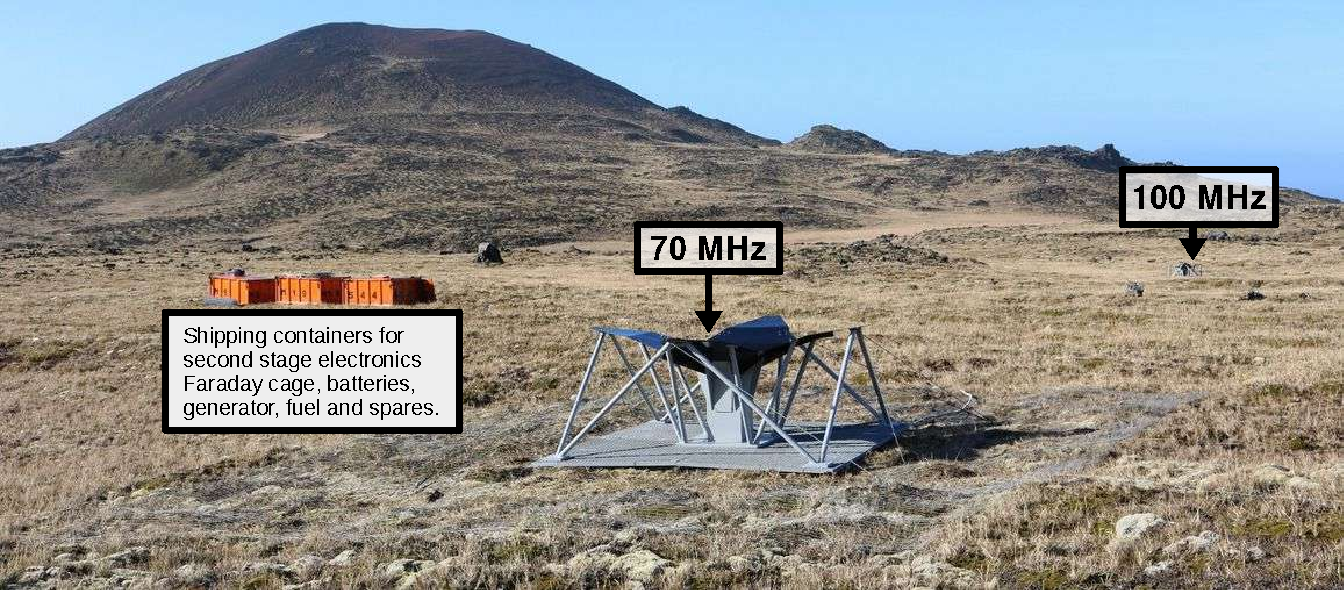
\includegraphics[width=\linewidth]{Figures/prizm.pdf}
	\caption{The \prizm\ experiment built on Marion Island. The two antennas (\SI{70}{\mega \hertz} and \SI{100}{\mega \hertz}) are visible and the the three shipping containers enclose the second stage electronics Faraday cage, generator, batteries, fuel, and spares. The main base lies four kilometers away from the observing site.}
	\label{Fig:prizm}
\end{figure}

\begin{figure}
	\centering
	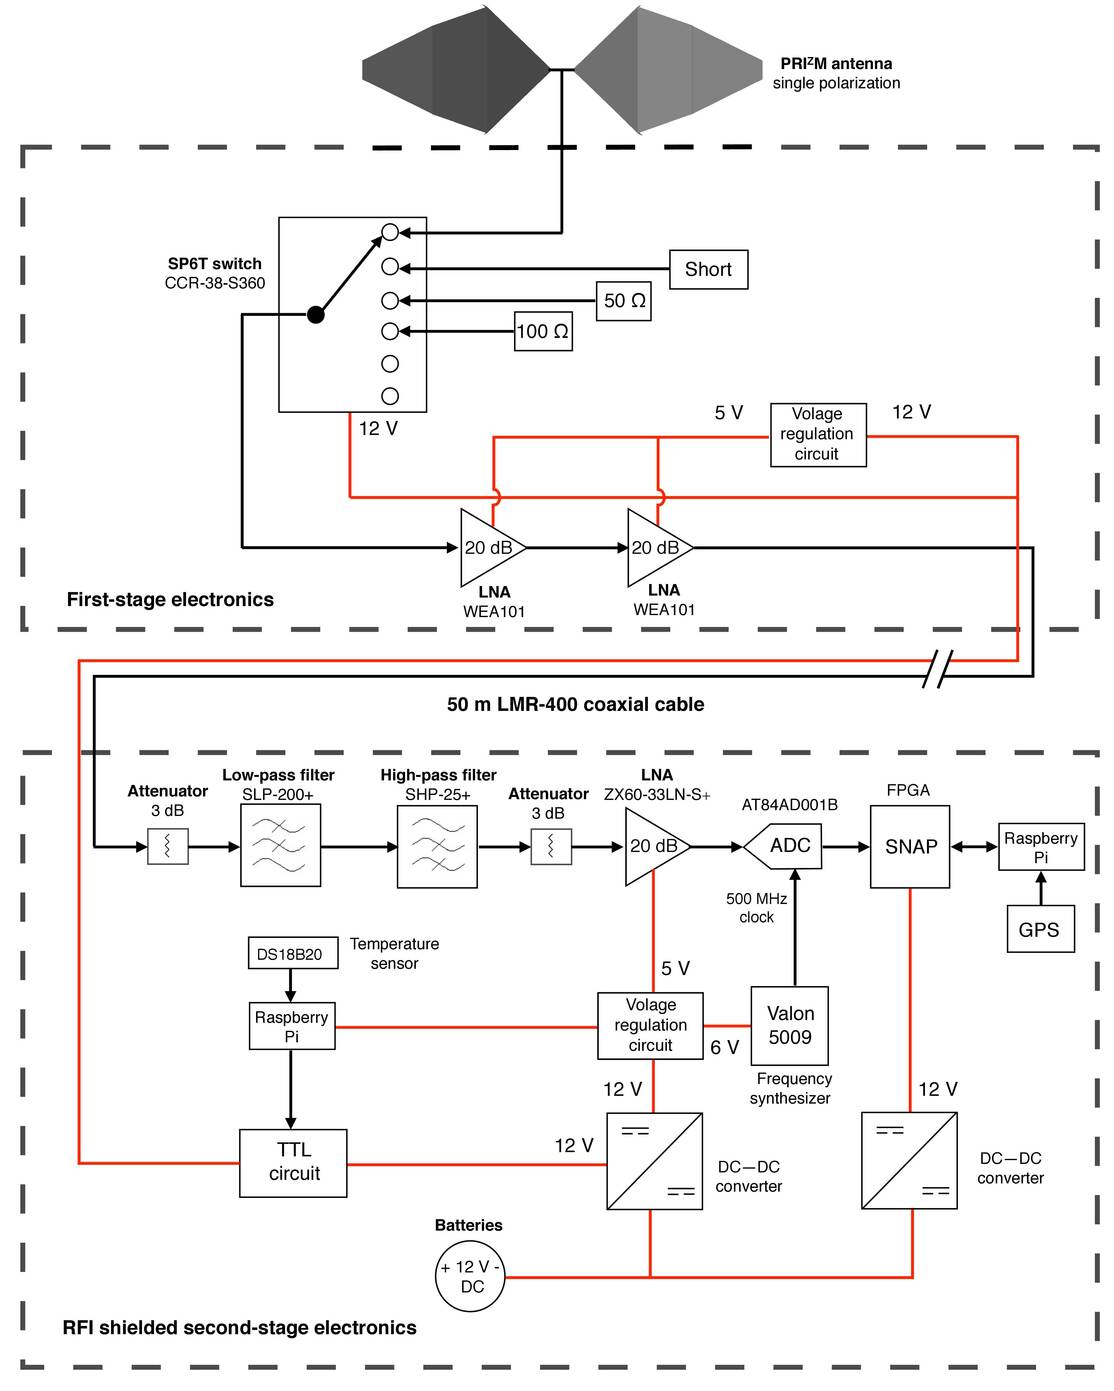
\includegraphics[width=\linewidth]{Figures/block_diagram}
	\caption{Block diagram for a single \prizm\ antenna polarization. The upper and lower dashed boxes denote the electronics chain's first and second stages. To decrease contamination from self-generated RFI, the 
		two stages are separated by \SI{50}{\meter}~\citep{2019JAI.....850004P}}. 
	\label{Fig:PRZIM_block}
\end{figure}

\section{Signal Chain}

\subsection{Antenna}

Figure~\ref{Fig:PRZIM_block} shows the original 2017 configuration of the signal chain for a single polarization of the \prizm\ antenna. The antenna design was initially developed for Sonda Cosmologica de las Islas para la deteccion de HIdrogeno neutro (SCI-HI), which was deployed in Guadalupe Island (\SI{200}{\kilo \meter} off the coast of Mexico) in 2013. The antenna is made up of four petals that form a pair of crossed dipoles. 

Each petal has three trapezoidal facets angled at various angles with respect to the ground. The angles were selected to minimize spectral variation in the beam shape. The antenna beam pattern's width has a direct dependence on the angles of the trapezoidal facets, and the height of the antenna above the ground changes the beam symmetry~\citep{2014ApJ...782L...9V}.  The \prizm\ antenna structure was redesigned with respect to the original SCI-HI design to survive the high winds on Marion Island, as shown in Figure~\ref{Fig:tel}.  


\begin{figure}
	\centering
	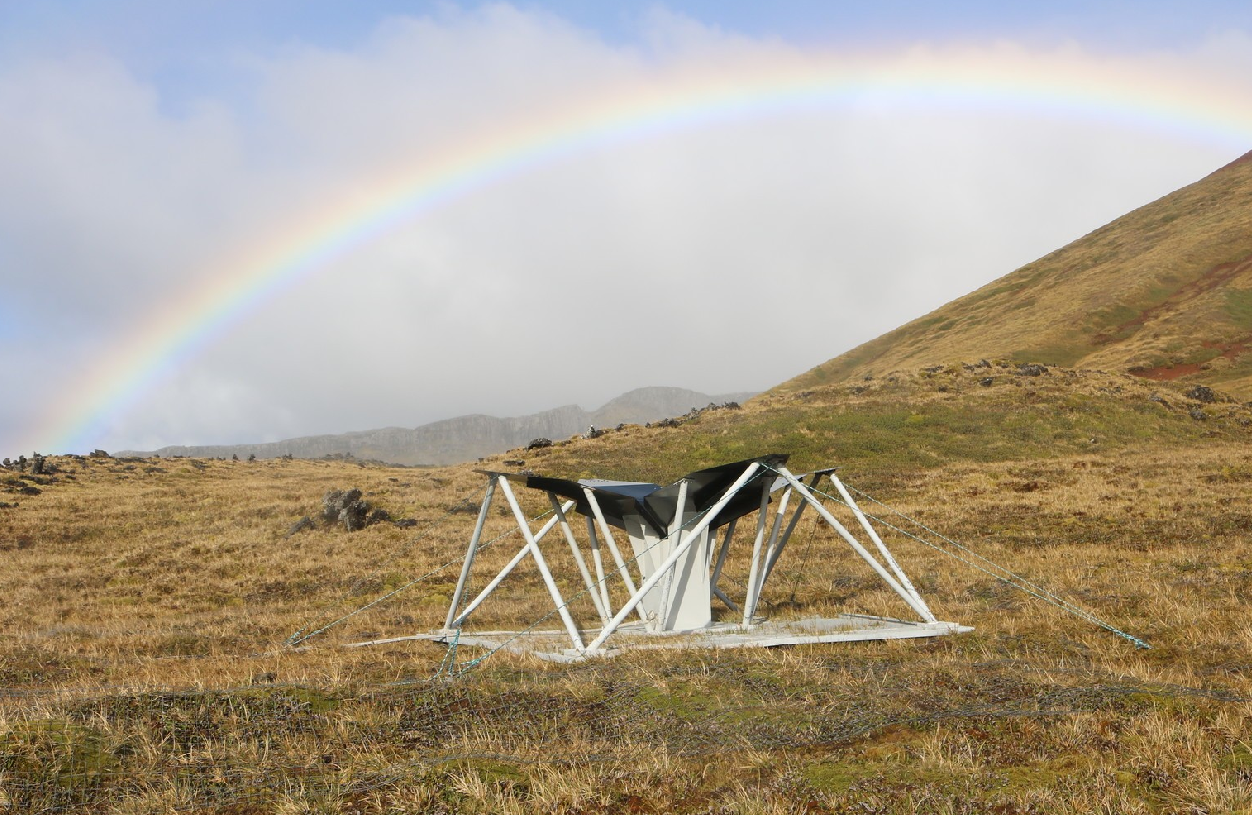
\includegraphics[width=\linewidth]{Figures/tel}
	\caption{A completed \SI{100}{\mega \hertz} antenna mounted on a \SI{2x2}{\meter} fibreglass grating with the approximate dimensions \SI{\sim 3}{\meter} on a side}.
	\label{Fig:tel}
\end{figure}

\subsection{First Stage Electronics}

The first stage electronics are housed in the column supporting the antenna petals as shown in Figure~\ref{Fig:column}, and the block diagram of the first stage electronics is shown in Figure~\ref{Fig:prizm_fee_block}. The signal from each single-polarization \prizm\ dipole is fed to the calibrator switch by a coaxial cable, which is \SI{200}{\milli \meter} long. In order to dissipate the current on the outer conductor of the coaxial cable, a ferrite core is used. The calibrator switch is required to switch between observations of the sky and the calibrator sources of \SI{50}{\ohm}, which are connected to the switch input terminals. Two cascaded WEA101 LNAs are used to amplify the selected signal at the switch output. Additional electronics in the first stage electronics box include voltage regulation circuitry for LNAs and temperature sensors. The two main improvements are upgrading to a latching switch from the 2017 to 2018 version, adding the noise source, and spreading thermometry through the components shown in Figure~\ref{Fig:prizm_fee_block}.

\begin{figure}
	\centering
	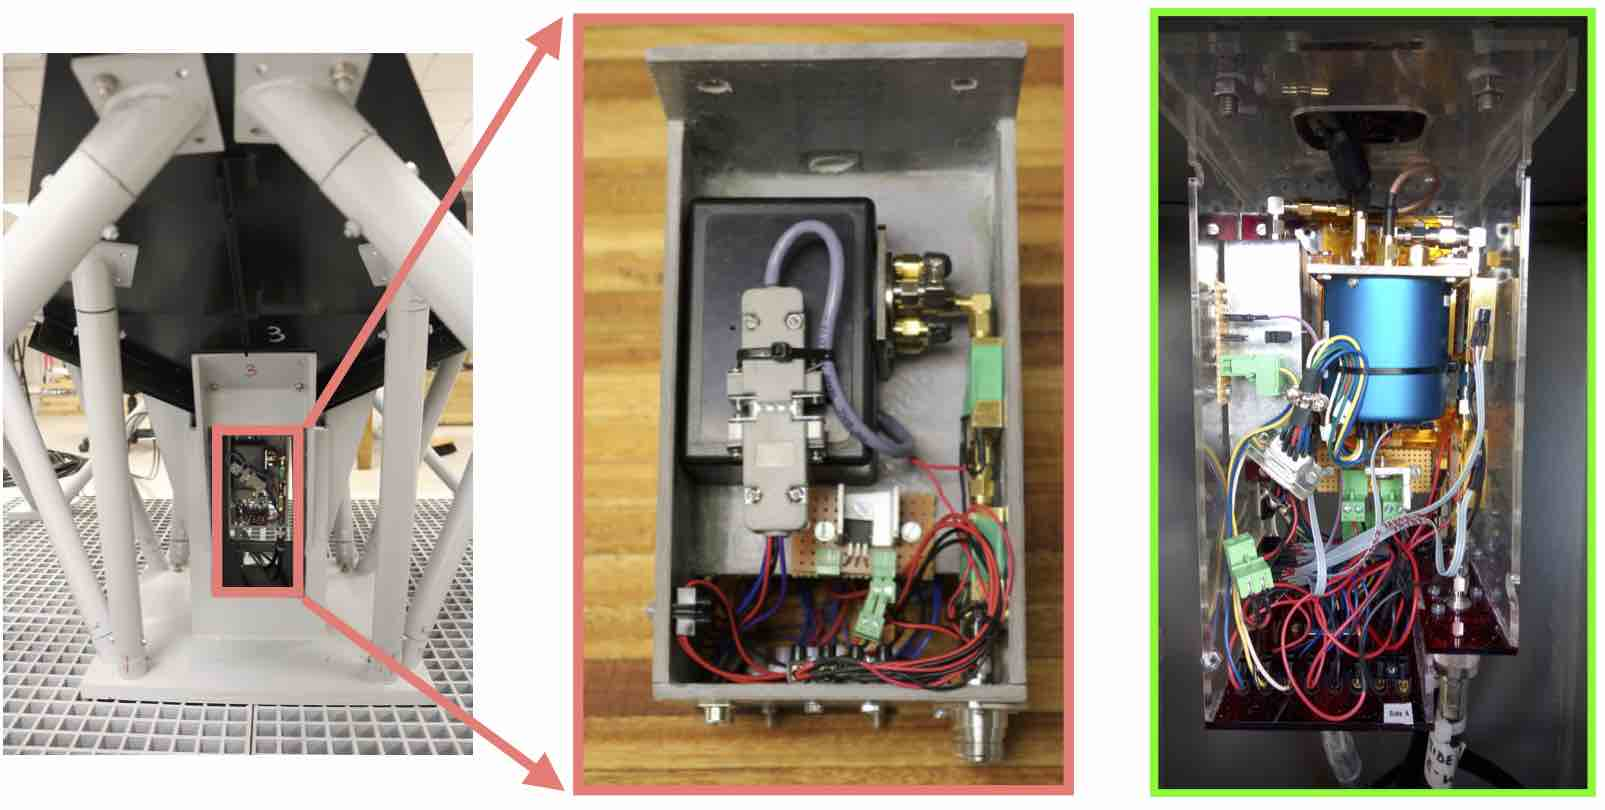
\includegraphics[width=0.7\linewidth]{Figures/column}
	\caption{The electronics box for the first stage. Shown in pink is the original installation from 2017 and green shows the 2018 upgrade which is currently installed in the central column under the antenna.}
	\label{Fig:column}
\end{figure}

\begin{figure}
	\centering
	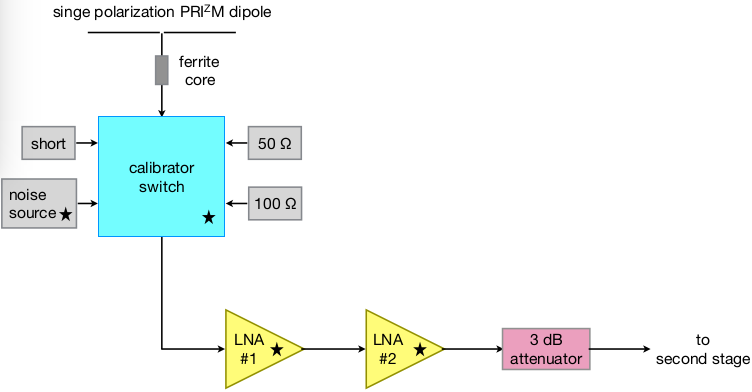
\includegraphics[width=\linewidth]{Figures/prizm_fee_block}
	\caption{A simplified schematic of electronics from the first stage. The schematic reflects the 2018 configuration. Components marked with a star are outfitted with one-wire digital temperature sensors.}
	\label{Fig:prizm_fee_block}
\end{figure}  

\subsection{Second Stage Electronics (SSE)}

A custom-designed Faraday cage (Figure~\ref{Fig:47093285614_63bb00be20_o}) that encloses the SSE is housed in one of the shipping containers shown in Figure~\ref{Fig:prizm}. The signal from the first stage electronics is fed via a \SI{\sim 50}{\meter} LMR400 coaxial cable, which is a reasonable distance to minimize the contamination from possible self-generated RFI. The coaxial cables are mouse-proofed using a few meters of stainless steel wire mesh cloth wrapped near the cable penetration points. The multi-tiered interior of the Faraday cage (\SI{\sim 300x470x240}{\milli \meter}) is shown in Figure~\ref{Fig:enclosure_ann} with the top panel removed. The readout box services both antennas. There is a separate readout chain for each antenna, but the housekeeping and switch control electronics are shared between the antennas. There are two central shelves for mounting the SNAP board and RPis. Each SNAP board services each antenna, and one RPi controls each SNAP. A third RPi is shared amongst the two SNAP boards for housekeeping purposes.

The filtering and amplification stage is applied to each polarization from each antenna. It consists of Minicircuits SLP-200+ and SHP-25+ low and high pass filters that band limit the RF signal to \SIrange{30}{200}{\mega \hertz}. The filtered signal is amplified by \SI{20}{\decibel} using a Minicircuits ZX60-33LN-S+ amplifier. The output signal is then fed to the readout electronics.

Each SNAP board receives the two RF signals from the two polarizations of a single antenna and samples the signals at a rate of \SI{500}{\mega samp\per \second} using a dual, monolithic, eight-bit, AT84AD001B external analog-to-digital converter (ADC) that is connected to the SNAP board via a Z-Dok connector. A Valon 5009 frequency synthesizer provides the ADC with a clock signal. The SNAP board employs a Xilinx Kintex 7 FPGA to compute auto- and cross- spectra from and between the four inputs, with 4096 frequency channels spanning 0--250~MHz. An RPi controls the SNAP board and saves data to an onboard SD-card. The RPi's timing is provided by an Adafruit Ultimate GPS module connected to an external active GPS antenna.

The SSE box also encloses the additional hardware that controls the calibrator switch states and voltage regulation. Figure~\ref{Fig:calibrator} shows the schematic of the switch control circuit. The L298 full-bridge drivers were used to make the control circuit, and the transistor-transistor-logic (TTL) is used to generate the control signals. Five L298 high-current full-bridge drivers are used to provide the reset and actuation signals. A power MOSFET is used to turn on and off a noise source in the FSE box. A Rpi controls the logic gates of the integrated chips. The whole first stage electronics is temperature monitored using the 1-wire DS18B20 temperature sensor.

\begin{figure}
	\centering
	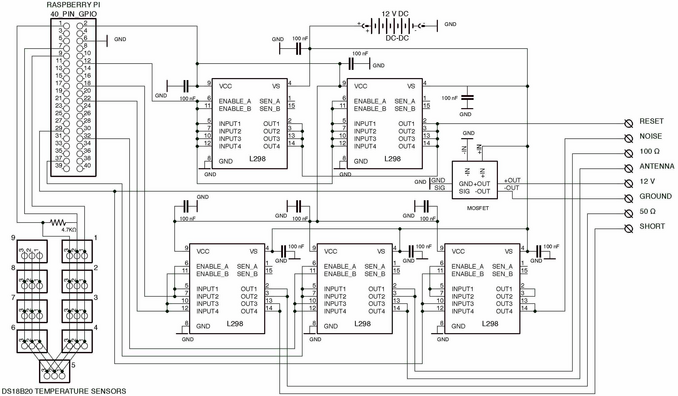
\includegraphics[width=\linewidth]{Figures/calibrator}
	\caption{The schematic of a switch control circuit. The L298 full-bridge drivers were used to make the control circuit. The two top drivers provide the reset signals, and the three bottom drivers provide actuation signals. To turn on and off the noise source in the FSE box, a power MOSFET is used. Nine 1-wire DS18B20 temperature sensors monitor the temperature.}
	\label{Fig:calibrator}
\end{figure}

The main power to the SSE box is fed via a BNC connector. The SSE box houses the two DC-DC converters on the bottom layer, which both provide \SI{12}{\volt} output, two SNAP boards are powered with \SI{12}{\volt} from one DC-DC converter. There are additional power regulators that input the \SI{12}{\volt} from the other DC-DC converter to supply lower voltage levels to multiple components in the system.

\begin{figure}
	\centering
	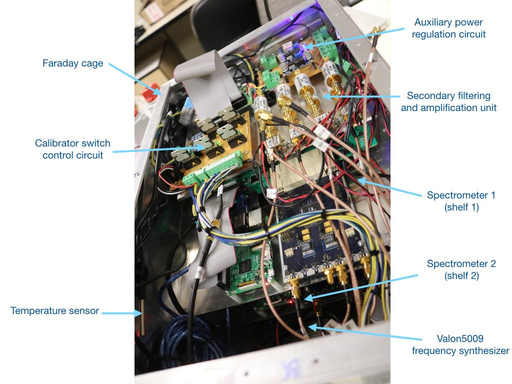
\includegraphics[width=0.7\linewidth]{Figures/enclosure_ann}
	\caption{The multi-tiered interior shown while the SSE box top panel is removed. Most of the internal components in this configuration can be accessed, but one more panel needs to be opened to access the DC-DC converters.}
	\label{Fig:enclosure_ann}
\end{figure}

\begin{figure}
	\centering
	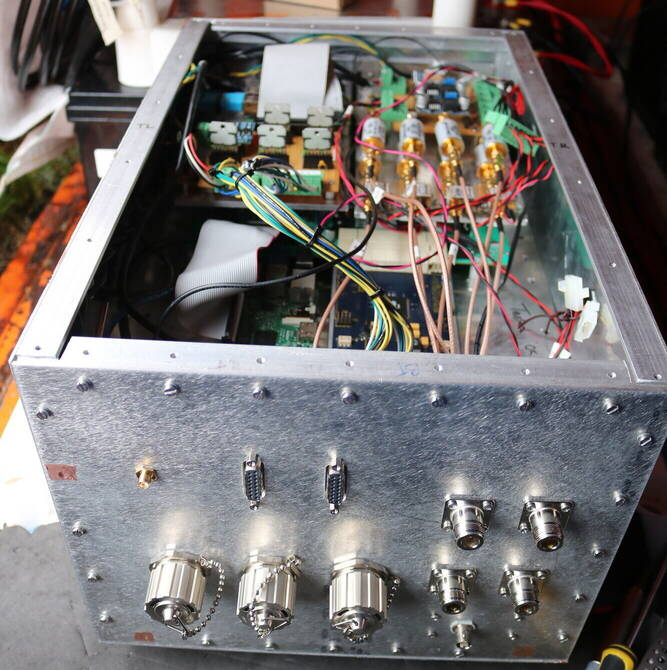
\includegraphics[width=0.4\linewidth]{Figures/47093285614_63bb00be20_o}
	\caption{The SSE Faraday cage made with separate brackets and flat sheets.}
	\label{Fig:47093285614_63bb00be20_o}
\end{figure}       

\subsection{Power}

The \prizm\ system is powered using eight \SI{12}{\volt} \SI{200}{\ampere \hour} battery bank wired in parallel as shown in Figure~\ref{Fig:power}. The total system draws \SI{\sim 65}{\watt} when the batteries are fully charged, the system can operate for approximately one week. Battery charging is performed manually using a Honda EU30is generator, and a fuel cache kept at the observing site. The batteries are connected to two DC/DC converters during observations. The DC-DC converters are enclosed in the SSE box and provides stable voltage outputs despite the slow decline of the battery voltage. Further regulation is performed to supply power to several components in the system.

\begin{figure}
	\centering
	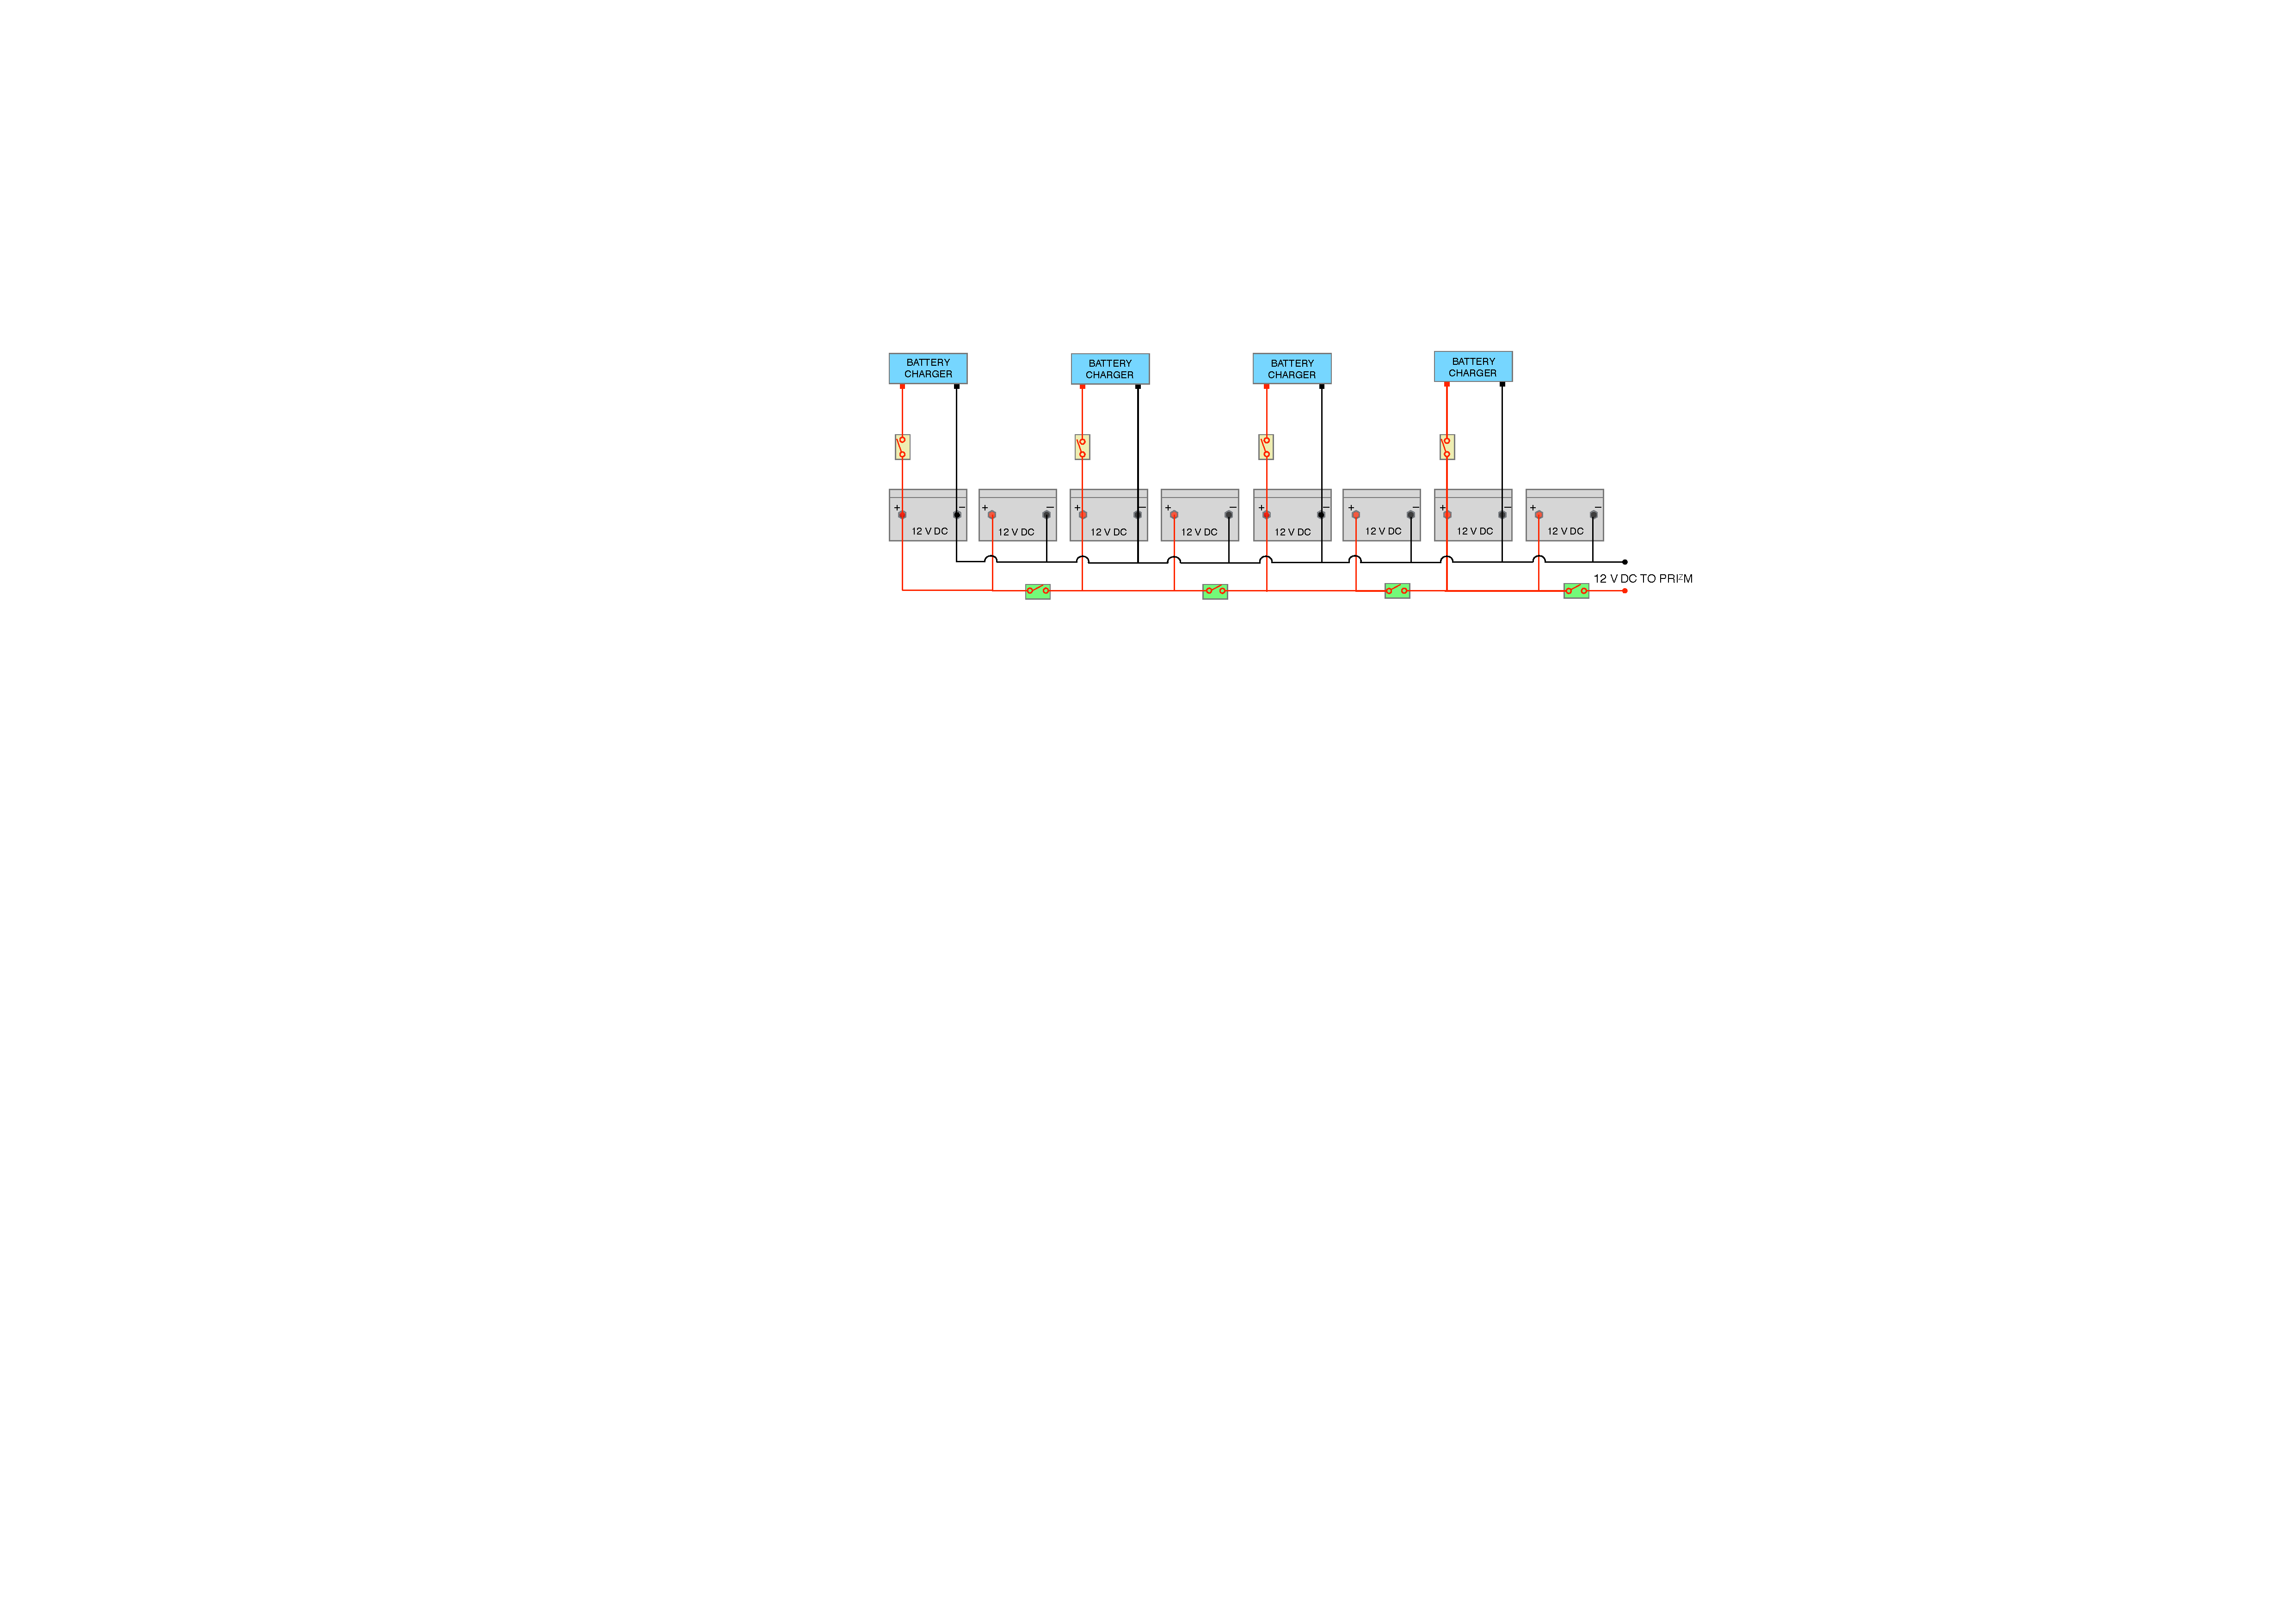
\includegraphics[width=\linewidth]{Figures/power_schematic}
	\caption{\prizm's power distribution chain consists of eight \SI{12}{\volt} \SI{200}{\ampere \hour} lead crystal batteries each. The batteries work in pairs that, through the green switches, are cascaded together. The battery pairs are disconnected during charging, and a single battery charger charges two batteries simultaneously. To connect the battery chargers, yellow switches are used. All yellow switches are turned OFF during the observation, and all green switches are powered ON.}
	\label{Fig:power}
\end{figure}

\section{Revised \prizm~Instrumentation}

This section describes revisions made to some of the \prizm\ subsystems in preparation for the 2020 voyage to improve functionality and performance. The first stage, electronics enclosure redesign, will be discussed in the next subsections and the revised SSE enclosure. Due to COVID-19 restrictions, the redesigned first stage electronics and SSE were not fully integrated and tested, and this section reports the work that was completed before lockdowns began. The 2020 Marion voyage was canceled because of COVID-19\footnote{\url{https://www.timeslive.co.za/news/south-africa/2020-04-06-sas-expedition-to-marion-island-downsized-over-coronavirus-fears/}}. 

\subsection{First Stage Electronics (FSE)}

A new FSE and enclosure were proposed for the 2020 deployment. Figure~\ref{Fig:FSE_rev} shows the block diagram of the proposed FSE architecture. Off-the-shelf enclosures were used instead of the previous enclosures' custom geometry, and these new boxes provide slightly more room to house the SPDT switches, which are new additions. To ensure that the enclosure would accommodate all the FSE, dummy placeholder components were crafted and placed in the enclosures. Figure~\ref{Fig:FSE_archi} shows a nominal component layout. The perforated gray sheet serves as a mechanical breadboard for easy addition of new parts without drilling the enclosures. Two enclosures are attached back to back to service the two polarizations. Most of the housekeeping electronics are on the side of Figure~\ref{Fig:FSE_archi}, which is intended to be accessed from the east-facing column door, giving the human slight shelter from the prevailing wind. The only housekeeping breakout on the second enclosure is half of the one-wire thermometry bus.

\begin{figure}
	\centering
	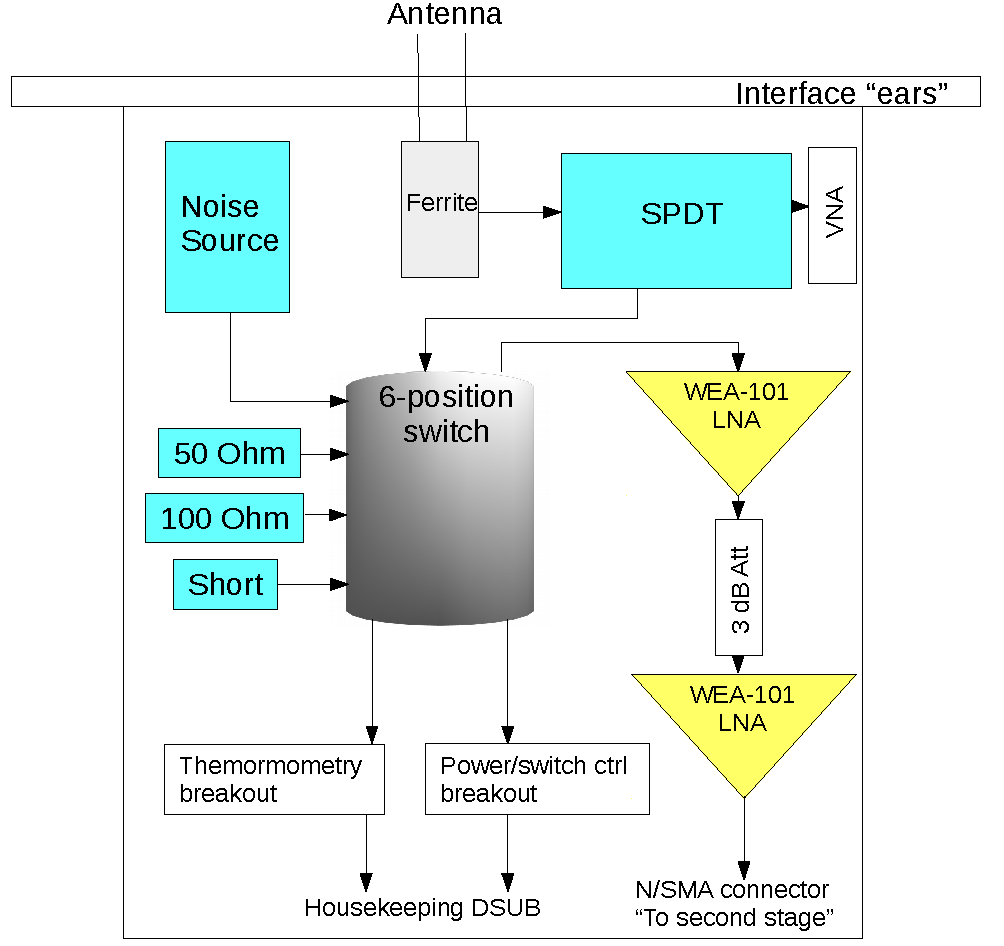
\includegraphics[width=0.7\linewidth]{Figures/FSE_rev}
	\caption{The block diagram of the proposed FSE achirtecture showing the 6-position switch connections, the breakouts for housekeeping, SPDT for controling the SP6T and amplification. The VNA is not permanently installed, and the box drawn indicates a connection point.}
	\label{Fig:FSE_rev}
\end{figure} 

The new box currently accommodates only one SPDT switch per side, and the plan is to add more switches to facilitate additional VNA measurements. The single SPDT switch does allow us to do VNA measurements of the antenna without disconnecting the antenna cables. The antenna cables connect the \prizm\ dipole to the calibrator switch. A right-angle adapter will be required on the SPDT to interface with the antenna cable. Without the SPDT switch in place, the S11 measurement looking into the antenna requires the antenna cable's physical disconnection from the 6-position switch. The new SPDT switch enables a selection of two positions, unlike the current \prizm\ configuration where the antenna signal is fed through the 6-position switch. The SPDT either selects the antenna signal to divert through the SPDT switch for VNA connection or continue as in the current configuration. In the new configuration, there is a free SMA port on the SPDT where the VNA can be connected or disconnected for measuring S11 looking into the antenna without connecting or disconnecting the cable. 

The terminal blocks for power and housekeeping signals have 16 positions total, so one is unused by the DB-15 breakout (and the SP6T switch can block the unused position). The filters in Figure~\ref{Fig:FSE_archi} are placeholders, but they are about the same size as the WEA-101 LNAs highlighted in yellow in Figure~\ref{Fig:FSE_rev}. In Figure~\ref{Fig:FSE_archi}, the incoming DB-15 connector is split out into two terminal blocks, and Table~\ref{Tab:Pinout} shows the connection configuration. The wall-mounted PCB has a 12V input and provides the LNAs with a 5V output and the one-wire thermometers with a 3.3V onboard output. All thermometers servicing both polarizations are ganged together on a single bus, so the headers are split accordingly across the enclosure's two halves.

\begin{figure}
	\centering
	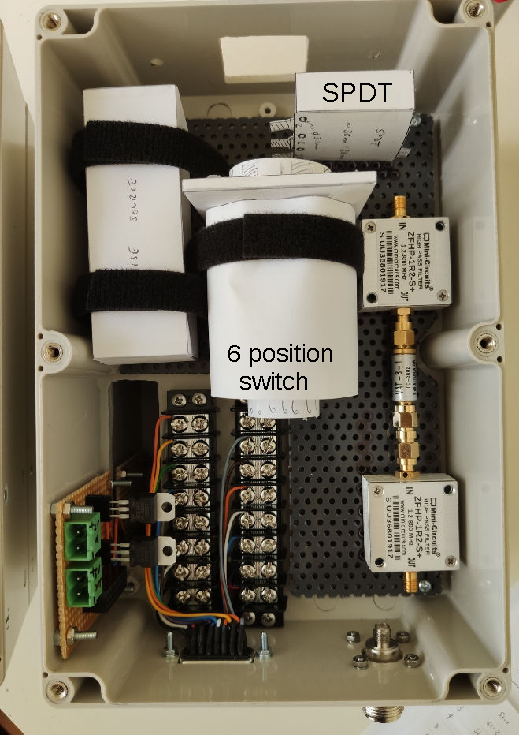
\includegraphics[width=0.5\linewidth]{Figures/FSE_archi}
	\caption{General layout of the components in the proposed FSE enclosure with dummy placeholders.}
	\label{Fig:FSE_archi}
\end{figure}

\begin{figure}
	\centering
	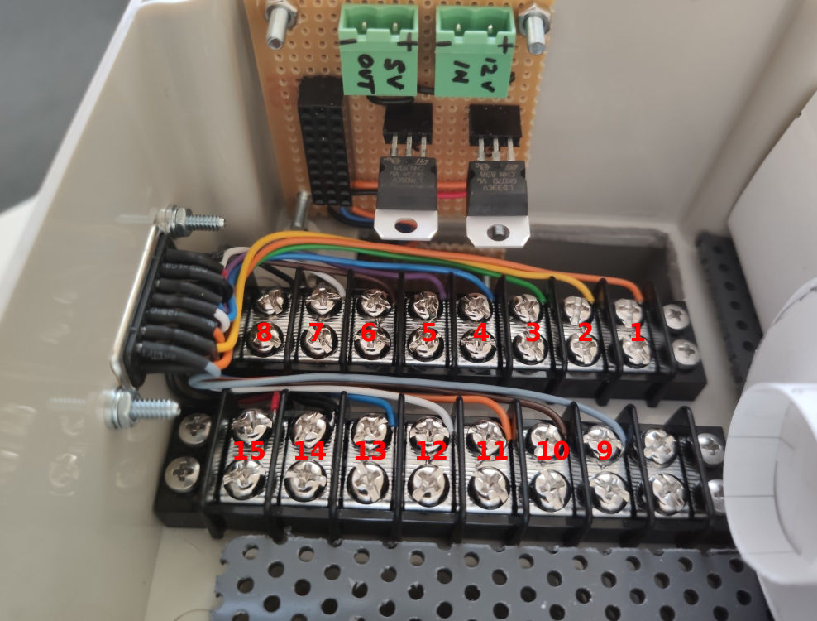
\includegraphics[width=0.7\linewidth]{Figures/Terminal}
	\caption{Housekeeping breakout. DB-15 pin assignments are annotated on the terminal blocks.}
	\label{Fig:Terminal}
\end{figure}

\begin{table}
	\centering
	\begin{tabular}{ c|c|c|c} 
		\hline
		DB-15 & Terminal Block & Colour & Function \\
		\hline
		\hline
		1 & L1 & Orange & S1-1 \\ 
		2 & L2 & Yellow & S1-2 \\ 
		3 & L3 & Green & S1-3 \\
		4 & L4 & Blue & S1-4 \\
		5 & L5 & Purple & S1-5 \\
		6 & L6 & Brown & S1-6 \\
		7 & L7 & White & S1-Reset \\
		8 & L8 & Black & Ground \\
		9 & R2 & Gray & S2-Ant \\
		10 & R3 & Brown & S2-Cal \\
		11 & R4 & Orange & Noise \\
		12 & R5 & White & Blank \\
		13 & R6 & Blue & Temp Sensor \\
		14 & R7 & Black & Ground \\
		15 & R8 & Red & 12 V \\
		\hline
	\end{tabular}
	\caption{Housekeeping pinout. Terminal block notation and numbering L and R denote left and right as viewed when the box is vertical, and numbers are from top to bottom. S1 denotes SP6T switch, S2 denotes SPDT switch.}
	\label{Tab:Pinout}
\end{table}


\subsection{Second Stage Electronics}

A revised Faraday cage for the SSE was designed using Autodesk Inventor Professional 2018, and the sheet metal box is shown in Figure~\ref{Fig:Enclosed}. The enclosure was revised so that each antenna has its SSE box.  There was no longer shared housekeeping RPi that binds the SNAP boards together. That was the main driver for separating the SNAP boards/ enclosures.

The switch circuit was redesigned as shown in Figure~\ref{Fig:newcontrol} by the schematic. Eight TLP3543 MOSFET output optocouplers were used to make the switch control circuit. Six of the optocouplers are used to control the 6-position switch, one is used for the reset, and the last one is used for the noise source. The circuit is designed to have a built-in precision real-time clock (RTC), and the chip used is the DS3231. Figure~\ref{Fig:control} shows the 3D view of the switch circuit PCB. The bigger green connector connects to the FSE via a DB15 connector mounted on the enclosure's front panel, and the smaller connector is for power distribution. Figure~\ref{Fig:Bottom} shows the female header, which is plugged directly into the RPi to form a stackable layout. The four mounting holes are precisely the same dimension as those of the RPi to fasten both of them simultaneously.

\begin{figure}
	\centering
	\includegraphics[width=\linewidth]{"Figures/new control"}
	\caption{Schematic diagram of the newly desined switch control circuit. In the new design, six out of eight MOSFET output optocouplers are used to control the 6-position switch, and the other two are used for reset and noise source. The circuit has a built-in RTC. RPi's GPIO pins are connected to the RTC and the optocouplers to controls the functionality.}
	\label{Fig:newcontrol}
\end{figure}


\begin{figure}
	\centering
	\begin{subfigure}[t]{0.52\textwidth}
		\centering
		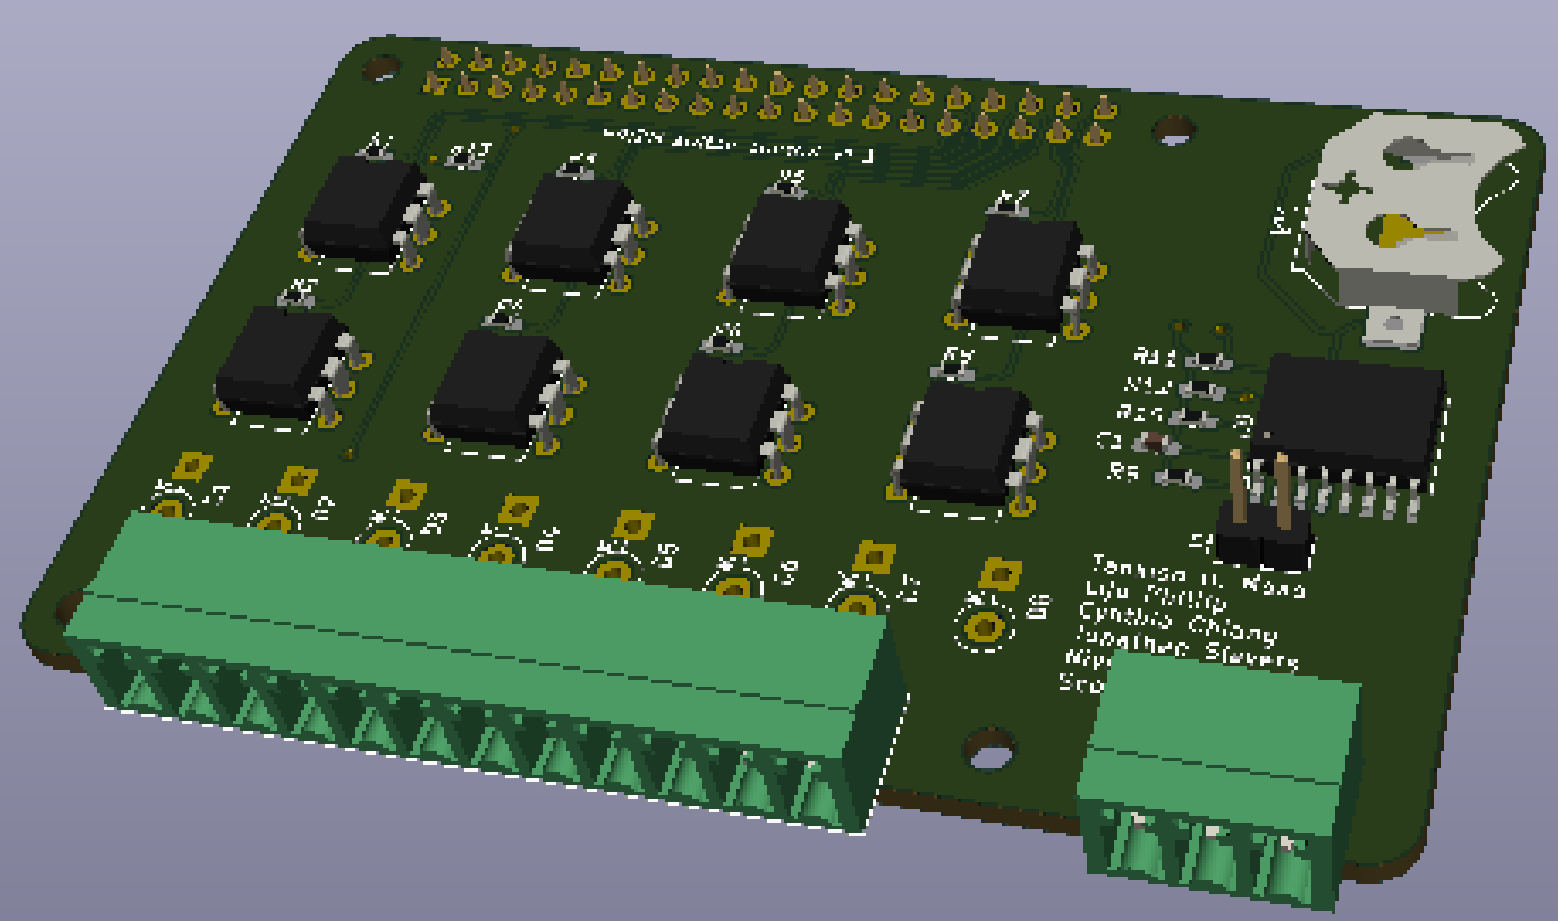
\includegraphics[width=\linewidth]{Figures/Top} 
		\caption{} \label{Fig:Top}
	\end{subfigure}
	\hfill
	\begin{subfigure}[t]{0.45\textwidth}
		\centering
		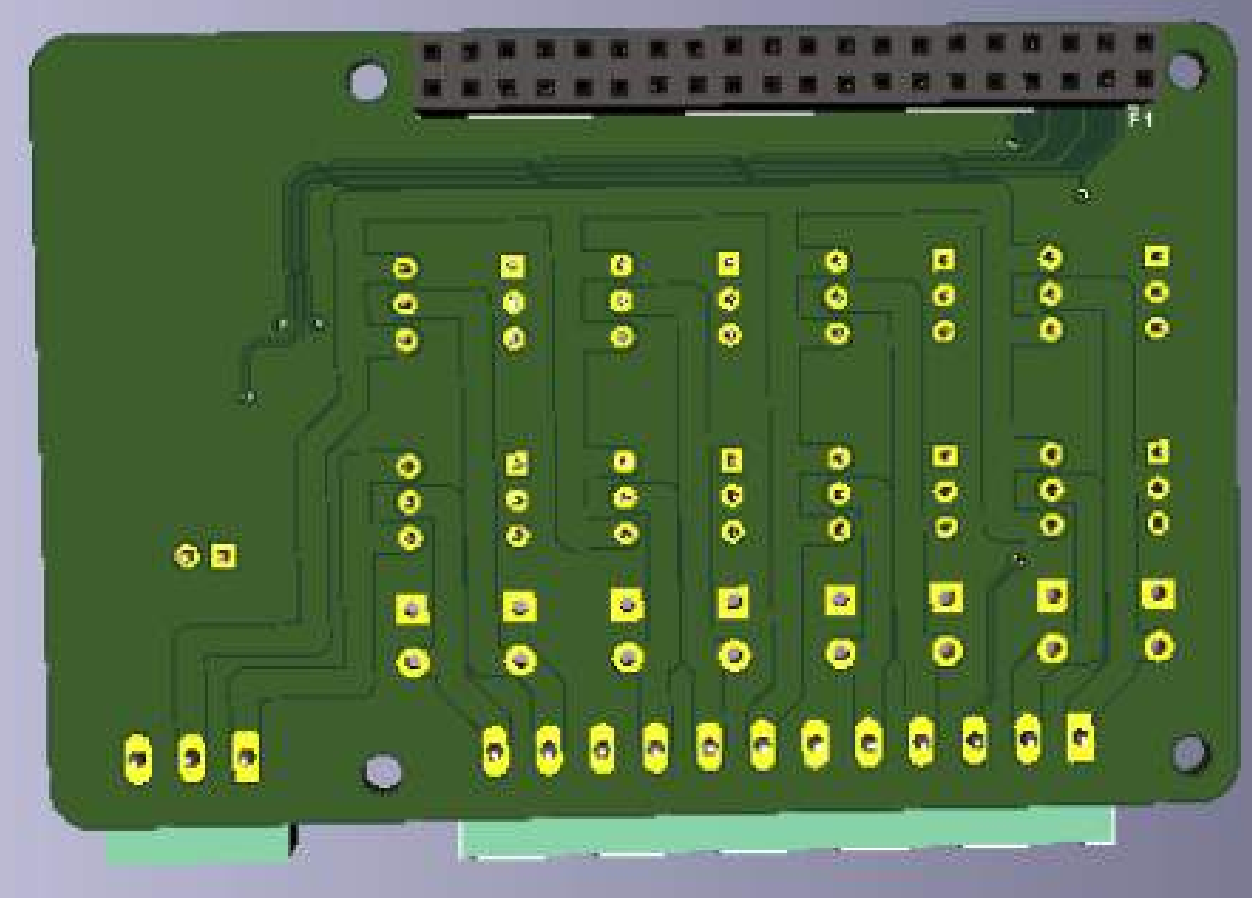
\includegraphics[width=\linewidth]{Figures/Bottom-compressed}
		\caption{} \label{Fig:Bottom}
	\end{subfigure}
	\caption{Top and bottom view of the newly designed switch control circuit. {\bf (a)} Top view. In the new design, six out of eight MOSFET output optocouplers are used to control the 6-position switch, and the other two are used for reset and noise source. {\bf (b)} Bottom view. The female header is connected to the GPIO pins of the RPi to form a stackable layout. The four mounting holes are exactly the same dimension as those of the RPi to fasten using taller fasteners.}
	\label{Fig:control}
\end{figure}

The main improvements to the new enclosure are listed below.

\begin{itemize}
	\item Increased and improved accessibility of all components. Because each enclosure now services only one antenna, all components can be accommodated on a single shelf that can be accessed from both sides.
	\item The design is folded laser cut sheet metal, unlike the separate brackets and flat sheets that make up the current design
	\item Easier and cheaper to assemble and manufacture
	\item User-friendly (the holes are already in place to tap and screw the components in place, and the lids are fastened using captive quarter-turn fasteners).
	\item It was designed to fit into a hiking backpack for easy carrying when hiking to the \prizm\ site. The current enclosure servicing both antennas is too large to carry on a hike to the site conveniently. The designed enclosure is \SI{\sim 400x280x110}{\milli \meter} and the current enclosure is \SI{\sim 300x470x240}{\milli \meter} 
	\item The new enclosure has a partitioned portion to accommodate the second stage RF electronics and ensure isolation from self-generated RFI from switching electronics elsewhere in the enclosure, as shown in Figure~\ref{Fig:Top Open}.
	\item A cooling fan was added to prevent thermal shutdowns of the SNAP board as shown in Figure~\ref{Fig:Bottom Open}.
	\item The switch control circuit was revised, and it is a stackable layout so that it sits on top of the RPi and connects directly to the GPIO pins.
	\item The RF absorbing material (3M Absorbing materials) is useful to line in the enclosure to avoid internal bounces from the RF noisy components, such as clocks of the digitizer and the switching from power supplies. That way, RFI is attenuated before reaching the amplifiers and other sensitive parts. 
\end{itemize}

A list of all components housed in the new enclosure is presented in Table~\ref{Tab:Components} with the quantities required. The front panel has feedthrough connectors that feed the signals/power in and out of the enclosure, as shown in Figure~\ref{Fig:Enclosed}. A non-isolated panel mount BNC connector is used to supply the main power to the box. Two N-F/SMA-F bulkheads (Amphenol 242163) are used for the second stage RF signals for both polarisations. Panel mount ethernet feedthrough (CONEC 17-101814) is for the data transfer between an enclosed RPi and the laptop. The filtered DB15 connector connects the FSE to the box.

\begin{table}
	\centering
	\begin{tabular}{ c|c}
		\hline
		Component & Quantity \\
		\hline
		\hline
		Meanwell 12VDC supply (RSD-60G-12) & 1 \\
		Terminal block for power breakout & 1 \\
		Buck converter & 2-4 \\
		Amplifier (ZX60-43-S+) & 2 \\
		High pass filter (HP-25+ HPF) & 2 \\
		Low pass filter (SLP-200+ LP) & 2 \\
		SNAP board	& 1 \\
		Switch control circuit & 1 \\
		Raspberry Pi 3, 3B+, or 4 & 1 \\
		Chronodot & 1 \\
		Adafruit GPS module & 1 \\		 
		\hline
	\end{tabular}
	\caption{A list of components that are housed inside the redesigned SSE enclosure.}
	\label{Tab:Components}
\end{table}

The enclosures were fabricated, and the sheet metal parts fitted together as designed, all the components were installed in the enclosures, and they fit the mounting holes that were already in place. COVID-19 lockdowns happened before dry-runs could be performed. 

\begin{figure}
	\centering
	\includegraphics[width=\linewidth]{"Figures/Top Open"} 
	\caption{CAD of an enclosure with the top lid open. The partioned portion is to avoid self-generated contamination from components with switching mechanisms. Some placeholders were mounted on the sheet metal design on Autodesk Inventor.} 
	\label{Fig:Top Open}
\end{figure}

\begin{figure}	
	\centering
	\includegraphics[width=\linewidth]{"Figures/Bottom Open"}
	\caption{The bottom view without the lid, showing the SNAP board and its cooling fan, and the RPi.} 
	\label{Fig:Bottom Open}
\end{figure}	

\begin{figure}
	\centering
	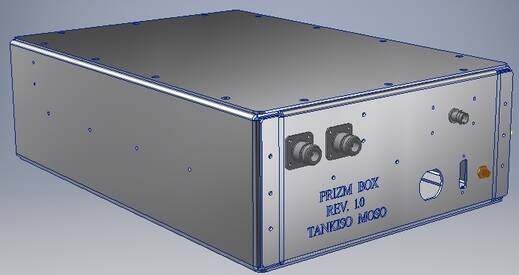
\includegraphics[width=\linewidth]{Figures/Enclosed}
	\caption{An enclosed box showing the connector placeholders and measured cutouts for other connectors that are not shown in this rendering}.	\label{Fig:Enclosed}
\end{figure}
